\documentclass[11pt]{article}
\usepackage[utf8]{inputenc}
\usepackage[T1]{fontenc}
\usepackage[french]{babel}
\usepackage{amsmath}
\usepackage[bookmarks={true},bookmarksopen={true}]{hyperref}
\usepackage{graphicx}
\usepackage[a4paper]{geometry}
\usepackage{listings}
\usepackage{amssymb}
\usepackage{amsmath,amsfonts}
	\lstset{frame=tb,
		language=Java,
 		aboveskip=3mm,
  		belowskip=3mm,
  		showstringspaces=false,
  		columns=flexible,
  		basicstyle={\small\ttfamily},
  		numbers=none,
 		numberstyle=\tiny\color{gray},
  		keywordstyle=\color{blue},
  		commentstyle=\color{dkgreen},
  		stringstyle=\color{mauve},
  		breaklines=true,
  		breakatwhitespace=true
  		tabsize=3
	}
\pagestyle{plain}
\setlength{\parindent}{5mm}
\usepackage{amsmath}
\usepackage{color}
\definecolor{dkgreen}{rgb}{0,0.6,0}
\definecolor{gray}{rgb}{0.5,0.5,0.5}
\definecolor{mauve}{rgb}{0.58,0,0.82}



\title{\textbf{Projet LSINF1121 -  Algorithmique et structures de données\\ - \\ Rapport intermédiaire Mission 4} \\ {\large Groupe 26}}
\author{Laurian \bsc{Detiffe} \\(6380-12-00)\and Sundeep \bsc{Dhillon} \\(6401-11-00)\and Alexis \bsc{Macq} \\ (5910-12-00) \and Xavier \bsc{Pérignon} \\ (8025-11-00)\and Thibaut \bsc{Piquard}\\(4634-13-00)\and Thomas \bsc{Wyckmans} \\ (3601-12-00)}
\date{date}
\date{\vspace*{25mm}

\includegraphics[scale=0.75]{logo.jpg}\\
		\vspace*{30mm}
		\begin{center}
		Année académique 2015-2016 \\	
		\end{center}}

\begin{document}
\thispagestyle{empty}

\maketitle
\thispagestyle{empty}
%\tableofcontents
%\setcounter{tocdepth}{3}
%\setcounter{page}{1}
%\newpage

\section*{Questions et réponses}
\begin{enumerate}
\item Citez au moins quatre implémentations différentes d’un dictionnaire (table de
symboles). Précisez, dans chaque cas, quelles sont les propriétés principales
de ces implémentations. Dans quel(s) cas s’avèrent-elles intéressantes ? Quelles
sont les complexités calculatoires de leurs principales méthodes ? (Xavier)\\
\begin{enumerate}
\item \textbf{Recherche séquentielle (liste désordonnée) :}

Une option simple pour la structure de données d'une table de symboles est une liste chaînée de noeuds qui contiennent des clés et des valeurs. Le principe de l'algorithme est qu'il parcourt la liste en comparant la clé de recherche avec la clé de chaque noeud dans la liste. Si les clés concordent, il retourne la valeur associée. Sinon, il retourne $null$. La mise en œuvre d'une liste liée à la recherche séquentielle est trop lente pour qu'elle puisse être utilisée pour résoudre d'énormes problèmes. Cependant, elle est idéale pour les petits problèmes.

\item \textbf{Binary tree search (BST) :}

Un arbre de recherche binaire est un arbre binaire où chaque noeud a une clé (et une valeur associée) et qui satisfait la restriction que la clé dans un noeud quelconque est plus grande que celle de tous les noeuds du sous-arbre gauche de ce noeud et plus petite que celle de tous les nœuds du sous-arbre droit de ce noeud. La mise en oeuvre de cette structure est très facile à implémenter. Cependant, si l'abre ressemble à une liste chaînée, cela risque d'augmenter fortement la complexité. 

\item \textbf{Separate chaining (tableau de listes) :}

Dans la méthode dite de chaînage séparé, chaque bucket est indépendant, et a une sorte de liste des entrées avec le même index. Le temps d'exécution d'une opération d'une table de hachage est le temps de trouver le bucket (qui est constant) plus le temps de l'opération concernant la liste. Dans une bonne table de hachage, chaque bucket a 0 ou 1 entrée, parfois 2 ou 3, mais rarement plus que cela. Par conséquent, les structures sont efficaces dans le temps et l'espace. Cependant, ce procédé hérite également les inconvénients des listes liées. En effet, lors du stockage de petites clés et de valeurs, la surcharge de l'espace du prochain pointeur dans chaque entrée peut être importante. 

\item \textbf{Linear probing (tableaux parallèles) :}

Linear probing est réalisée en utilisant deux valeurs : une étant comme une valeur de départ et une autre étant comme un intervalle entre les valeurs successives en arithmétique modulaire. La seconde valeur, qui est la même pour toutes les clés et connue sous le nom $stepsize$, est ajoutée à plusieurs reprises à la valeur de départ jusqu'à ce qu'un espace libre est trouvé, ou que toute la table soit parcourue.
\begin{center}
$newLocation = (startingValue + stepSize) \% arraySize$
\end{center}
Cet algorithme offre une bonne mise en cache de la mémoire (si $stepsize$ est égal à 1), grâce à la bonne localité de référence.\\
\end{enumerate}
\textbf{Résumé :}
\begin{center}
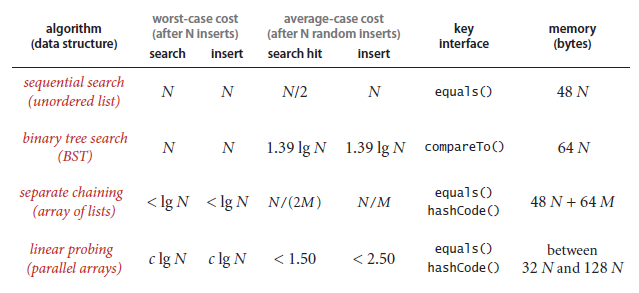
\includegraphics[scale=0.75]{symbol.PNG}
\end{center}
\item Souvenez vous de la question suivante proposée en bilan sur la mission sur les
tris : Étant donné un ensemble $S$ de taille $n$, et un nombre $x$. Décrivez un algorithme
efficace utilisant une HashTable pour trouver s’il existe une paire $(a, b)$
avec $a \in S$, $b \in S$ telle que $a + b = x$. Quelle est la complexité de votre algorithme
? Est-elle meilleure que votre solution qui utilisait un tri ? (Xavier)\\

Concernant le bilan sur la mission sur les tris, la solution était de faire un tri efficace de l'ensemble $S$ (par exemple Quicksort) et ensuite de tester l'addition du premier élément $a$ avec le dernier élément $b$. Si le résultat de cette addition était inférieur à $x$, alors on testait l'addition de $(a+1)$ avec $b$, et ainsi de suite. Sinon si le résultat de l'addition était supérieur à $x$, alors on testait l'addition de $a$ avec $(b-1)$, et ainsi de suite.\\\\
Pour résoudre le même problème avec une HashTable, on pourrait penser à insérer tous les éléments de l'ensemble $S$ dans une HashSet. Cette classe implémente l'interface Set, en utilisant une HashTable. HashSet est implémenté comme une HashMap, dont les clés sont les éléments du HashSet et les valeurs sont toutes une même valeur présente. Cette implémentation offre des performances constantes pour les opérations \textit{add(T t)}, \textit{remove(T t)}, \textit{contains(T t)} et \textit{size()}. Il suffira donc de vérifier si pour chaque élément $a$ de l'ensemble $S$, il existe $b$ dans la HashSet tel que $b = x - a$. La complexité de cet algorithme est donc de $O(1)$ + $O(n)$ (parcours des éléments de $S$). Ce qui est plus rapide que l'algorithme de la mission sur les tris.\\

\item Démontrez que $(a + b)\%M$ est équivalent à $((a\%M) + b)\%M$. En quoi cette 
propriété peut être utile pour construire une fonction de hachage sur les String.
Expliquez comment Java calcule une fonction de hachage sur les String ? Quelle
est la complexité pour calculer 1 fois et N fois le hashcode d’un String. (Xavier)\\

Prenons G = $(a + b)\%M$ et D = $((a\%M) + b)\%M$.\\ 
On doit démontrer que G = D.\\
Nous pouvons écrire :
\begin{center}
a = M * Q1 + R1 where 0 $\le$ R1 < M où Q1 est un entier. a mod M = R1\\
b = M * Q2 + R2 where 0 $\le$ R2 < M où Q2 est un entier. b mod M = R2\\
(a + b) = M * (Q1 + Q2) + R1+R2 \\
G = (a + b) mod M\\
G = (M * (Q1 + Q2) + R1+ R2) mod M\\
\end{center} 
On peut supprimer les multiples de M lorsqu'on prend mod M,
\begin{center}
G = (R1 + R2) mod M\\
D = (a mod M + b) mod M\\
D = (R1 + R2) mod M\\
\end{center}
Et donc, 
\begin{center}
G = D = (R1 + R2) mod M\\
\end{center}
\vspace{1\baselineskip}
Cette propriété est utile pour construire une fonction de hashage sur les String car il n'est pas nécessaire de calculer le modulo de chaque valeur des caractères du String. En effet, il suffira de calculer la somme de la valeur des caractères et utiliser une seule fois le modulo à la fin.\\\\
La fonction de hashage pour un String est implémentée comme suit :
\begin{center}
$s[0]*31^{(n-1)} + s[1]*31^{(n-2)} + ... + s[n-1]$
\end{center}
Dans cette fonction, le String $s$ a $n$ caractères. Elle calcule la somme des valeurs de chaque caractère, chacun multiplié par $31^{r}$ avec $r$ étant l'emplacement inversé du caractère dans le String. La complexité du calcul de hashcode d'un String est de $O(n)$ puisqu'il faut parcourir tous les caractères du String. Mais une fois ce calcul fait, il n'est plus nécessaire de recalculer le hashcode de ce String.\\

\item
\item Java fournit la classe \texttt{java.util.Hashtable} comme implémentation de l'interface \texttt{java.util.Map}. Pouvez-vous déterminer précisément de quelle variante de table de hachage il s'agit ? Java fournit-il d'autres implémentations de l'interface \texttt{Map} ? Faites un diagramme qui représente les interfaces et les classes qui se rapportent à \texttt{Map} et précisez ce qui, dans chaque cas, les caractérise. Qu'est-ce qui peut servir de clef pour une \texttt{Hashtable} en Java ? Soyez précis. (Sundeep) \\

En Java, on a plusieurs implémentations de l'interface \texttt{java.util.Map} et vous trouverez ci-dessous un schéma simplifié avec les interfaces et les classes qui se rapportent à l'interface \texttt{java.util.Map}:
\begin{figure}
\center
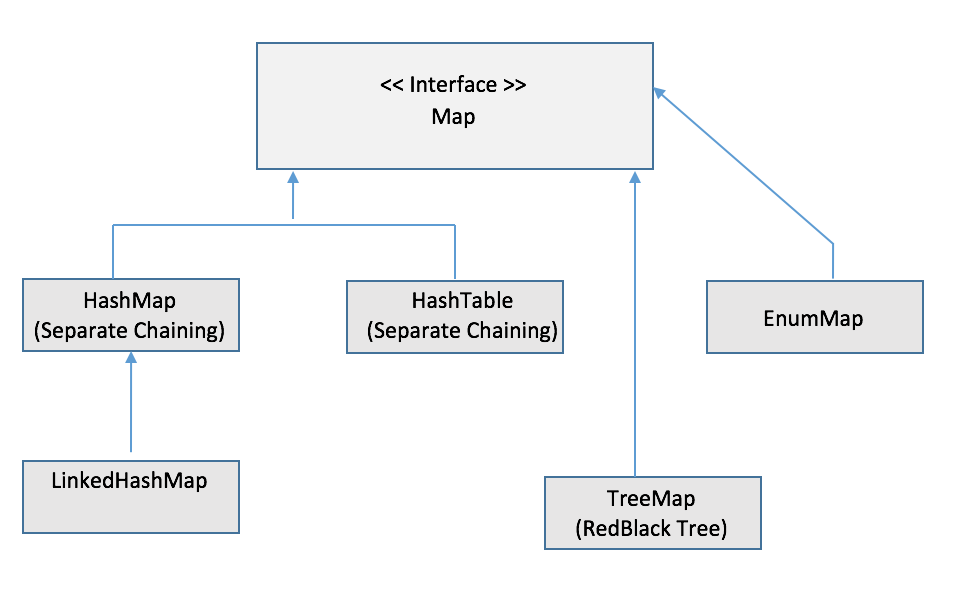
\includegraphics[scale=0.8]{diag.png}
\end{figure}

\begin{itemize}
\item La différence entre HashMap et HashTable est que l'un n'est pas synchronisé alors que l'autre, oui (donc HashTable est thread-safe) et une autre différence est le fait qu'un HashTable n'accepte pas les clés ou valeurs \textit{null} alors qu'un HashMap accepte au maximum une clé valant \textit{null} et le nombre de valeurs null que l'on souhaite.
\item LinkedHashMap utilise une liste doublement chaînée. On peut donc itérer sur un LinkedHashMap en gardant l'ordre de l'insertion des clés dans le LinkedHashMap.
\item EnumMap est une implémentation d'un Map qui utilise des clés qui ont comme type un Enum Java. C'est efficace car on n'utilise qu'un seul objet Enum spécifié lors de l'initialisation de l'EnumMap.
\item TreeMap utilise une implémentation d'un RedBlack Tree pour garder les clés triées selon leur ordre naturel.
\end{itemize}

\item Qu'entend-on par la notion de collision dans une table de hachage ? Les collisions ont-elles une influence sur la complexité des opérations ? Si oui, quelle(s) opération(s) avec quelle(s) complexité(s), sinon précisez pourquoi. (Thomas)\\

Le fait de créer une valeur de hachage à partir d'une clé peut engendrer un problème de « collision », c'est-à-dire que deux clés différentes, voire davantage, pourront se retrouver associées à la même valeur de hachage et donc à la même case dans le « tableau » (la fonction n'est pas injective). Pour diminuer les risques de collisions, il faut donc premièrement choisir avec soin sa fonction de hachage. Ensuite, un mécanisme de résolution des collisions sera à implémenter.\\
Tout comme les tableaux ordinaires, les tables de hachage permettent un accès en O(1) en moyenne, quel que soit le nombre d'éléments dans la table. Toutefois, comme plusieurs données peuvent se trouver dans une même case, le temps d'accès dans le pire des cas peut être de O(n). Comparées aux autres tableaux associatifs, les tables de hachage sont surtout utiles lorsque le nombre d'entrées est très important





\item Qu'est-ce que le facteur de charge d'une table de Hashage? Est-ce que le contrôle du facteur de charge est nécessaire/optionnel pour le bon fonctionnement d'une table de Hashage avec Linear Probing ou Separate Chaining ? Quelle est la stratégie utilisée par \texttt{java.util.Hashtable} pour contrôler le facteur de charge ? En quoi est-elle différente de celle proposée dans \texttt{LinearProbinHashST} ? Quel est le lien entre le facteur de charge et collision ? (Sundeep) \\


Le facteur de charge d'une table de hachage correspond au ratio $\alpha = \frac{N}{M} $  avec N étant le nombre d'éléments présents dans cette table et M, la taille de la table. 

Que ce soit pour le Linear Probing ou le Separate Chaining, il est important de bien contrôler le facteur de charge pour le bon fonctionnement d'une table de Hashage. Dans le cas du Separate Chaining, le facteur de charge correspondra au nombre moyen de clés par listes et donc, il sera souvent supérieur à 1. Dans le cas du Linear Probing, le facteur de charge correspondra au taux d'entrées remplies dans la table et ne fonctionne plus lorsqu'on atteint 1. Pour palier à ce problème, on effectue un resizing (souvent, on créé une table deux fois plus grande et on la remplir avec les élements de l'ancienne). \\
\texttt{java.util.Hashtable} utilise la méthode dont on vient de parler.\\
La différence principale entre les stratégies de redimensionnement de \texttt{Hashtable} et \texttt{LinearProbingHashST} est que cette dernière redimensionne vers une taille plus petite quand la charge du tableau devient plus petite (quand le tableau est seulement un huitième plein). De cette manière, elle peut assurer que l'espace occupé par la table sera toujours proportionnel à son contenu.


Il existe un lien entre la notion de collision et le facteur de charge, à  savoir: plus le facteur de charge est grand, plus le tableau est rempli et par conséquent, plus le risque de collisions augmente.


\item Imaginez une nouvelle méthode \texttt{iterator()} qui retourne un itérateur sur les clefs de \texttt{LinearProbingHashST}. Votre itérateur ne devrait pas accepter de modification de la table de hashage alors qu'il est utilisée :
une \texttt{ConcurrentModificationException()} doit être lancée si c'est le cas. Que suggérez-vous pour ce faire ? Hint : Inspirez vous de la stratégie de \texttt{java.util.Hashtable}. (Thomas)\\

Iterator() parcoura la table de Hashage des clés jusqu'à M, en retournant à chaque fois la clés attendu grâce a la méthode next(). Il est bien évident qu'il contiendra les méthodes hasnext() qui lui indiquera si il y a encore un élément à lire après. Toutefois, si lors de l'appel à la méthode next(), le flag de modification est mise à vrai, Iterator() enverra ConcurrentModificationException().

\item 
\item \textbf{Fonction de hash permettant de calculer le hachage du sous-string[i+1,...,i+n] en temps constant en connaissant le hachage du sous-string[i,...,i+n-1]} (Alexis)\\

Une fonction de hashage qui utilise une méthode de Horner peut permettre d'implémenter
l'opération voulue.
Voici cette fonction de hash :

\begin{lstlisting}

private long quick_next_string_hash(String txt_to_hash, int n, int i)
{
\end{lstlisting}
	// Initialisation
\begin{lstlisting}
	long hash = 0;
	int prime_to_modulo = 997;
	int R = 100;
	int j;
	
	for(j = 0; j < M; j++){
		pre_hash = R*hash + key.charAt(i+j);
		hash = (R*hash + key.charAt(i+j)) % prime_to_modulo;
	}
\end{lstlisting}
	/* Utilisons la notation t\_i pour s.charAt(i). On voit ici que le sous-string \\
	 * $ s[i,...,i+n-1] = t_{i}*R^{n-1} + t_{i+1}*R^{n-2} + ... + t_{i+n-1}*R^{0} $ \\
	 * peut nous donner en une seule opération, le sous\_string s[i+1,...,i+n]. \\
	 * En effet, on peut facilement obtenir l'égalité suivante \\
	 * $ x_{i+1} = (x_{i} - t_{i}*R^{n-1})*R + t_{i+n} $ \\
	 */ Cette opération étant complexe, séparons-là en 2 opérations plus simples. \\
	\\
	// Commençons par retirer le $ t_{i}*R^{n-1} $
\begin{lstlisting}
	long quick_next_string_hash = (hash + prime_to_modulo - R^{n-1}*txt_to_hash.charAt(i) % prime_to_modulo) % prime_to_modulo;

\end{lstlisting}
	// Ajoutons la contribution du nouveau caractère au hash après avoir multiplié par R
\begin{lstlisting}
	quick_next_string_hash = (quick_next_string_hash*R + txt_to_hash.charAt(i+n)) % Q;
	
	return quick_next_string_hash;
}

\end{lstlisting}

\item \textbf{Rechercher des sous-strings de tailles différentes via une fonction de hashage} (Alexis)\\

On utilise l'algorithme de Rabin-Karp que voici telle que dans le livre de référence :

\begin{lstlisting}

public class RabinKarp
{
	private String pat; // pattern (only needed for Las Vegas)
	private long patHash; // pattern hash value
	private int M; // pattern length
	private long Q; // a large prime
	private int R = 256; // alphabet size
	private long RM; // R^(M-1) % Q
	public RabinKarp(String pat)
	{
		this.pat = pat; // save pattern (only needed for Las Vegas)
		this.M = pat.length();
		Q = longRandomPrime(); // See Exercise 5.3.33.
		RM = 1;
		for (int i = 1; i <= M-1; i++) // Compute R^(M-1) % Q for use
			RM = (R * RM) % Q; // in removing leading digit.
		patHash = hash(pat, M);
	}
	public boolean check(int i) // Monte Carlo (See text.)
	{ return true; } // For Las Vegas, check pat vs txt(i..i-M+1).
	private long hash(String key, int M)
	{ // Compute hash for key[0..M-1].
		long h = 0;
		for (int j = 0; j < M; j++)
			h = (R * h + key.charAt(j)) % Q;
		return h;
	}
	private int search(String txt)
	{ // Search for hash match in text.
		int N = txt.length();
		long txtHash = hash(txt, M);
		if (patHash == txtHash) return 0; // Match at beginning.
		for (int i = M; i < N; i++)
		{ // Remove leading digit, add trailing digit, check for match.
			txtHash = (txtHash + Q - RM*txt.charAt(i-M) % Q) % Q;
			txtHash = (txtHash*R + txt.charAt(i)) % Q;
			if (patHash == txtHash)
				if (check(i - M + 1)) return i - M + 1; // match
		}
		return N; // no match found
	}
}

\end{lstlisting}

Si on a des strings de taille M1, M2, ..., Mk à rechercher dans un long string M,
on peut prendre toutes les sous-strings de début des strings de la taille du plus 
petits des strings $ M_{i} \forall i $.
Dès qu'on a un match, on utilise la fin de la fonction expliquée à la question précédente
pour vérifier que la fin du string match aussi. Une telle fonction reste en $ O(n) $.


\end{enumerate}
\end{document}